\documentclass{article}

\usepackage[catalan]{babel}
\usepackage{translations}
\usepackage[titles]{tocloft}
\usepackage{multicol}
\usepackage{graphicx} % Required for the inclusion of images
\usepackage{amsmath} % Required for some math elements 
\usepackage{hyperref}
\usepackage{amsmath}
\usepackage{listings}
\usepackage{courier}
\usepackage[margin=1in]{geometry}
\usepackage{changepage}
\usepackage{titlesec}
\usepackage{wrapfig}
\usepackage[version=4]{mhchem}
\usepackage{multirow}
\usepackage{siunitx}
\usepackage{ragged2e}
\usepackage{adjustbox}
\usepackage{caption}
\usepackage[table,xcdraw]{xcolor}


\definecolor{codegreen}{rgb}{0,0.6,0}
\definecolor{codegray}{rgb}{0.5,0.5,0.5}
\definecolor{codepurple}{rgb}{0.58,0,0.82}
\definecolor{backcolour}{rgb}{0.95,0.95,0.92}

\lstdefinestyle{mystyle}{
    backgroundcolor=\color{backcolour},   
    commentstyle=\color{codegreen},
    keywordstyle=\color{magenta},
    numberstyle=\tiny\color{codegray},
    stringstyle=\color{codepurple},
    basicstyle=\ttfamily\footnotesize,
    breakatwhitespace=false,         
    captionpos=b,                    
    keepspaces=true,                 
    numbers=left,                    
    numbersep=5pt,                  
    showspaces=false,                
    showstringspaces=false,
    showtabs=false,                  
    tabsize=2
}
\lstset{language=Python, 
        basicstyle=\ttfamily\small, 
        keywordstyle=\color{keywords},
        commentstyle=\color{comments},
        stringstyle=\color{red},
        showstringspaces=false,
        identifierstyle=\color{codepurple},
        keywords=[2]{pow},
        keywordstyle=[2]{\color{orange}},
}

\lstset{style=mystyle}
\setlength\parindent{0pt}
\renewcommand{\labelenumi}{\alph{enumi}.}

\setlength\parindent{0pt} % Removes all indentation from paragraphs

\renewcommand{\labelenumi}{\alph{enumi}.} % Make numbering in the enumerate environment by letter rather than number (e.g. section 6)
   
\newcommand{\titulo}{Determinació de l'entalpia \\de vaporització de l'aigua}
\newcommand{\nombreestudiante}{Víctor Mira Ramírez}
\newcommand{\nombredirector}{Ángel Ávila Freire}
\newcommand{\fecha}{\date{Març 2023}}  % Definir solo el año de presentación

\pagebreak

\renewcommand{\listtablename}{Índex de taules} 
\renewcommand{\tablename}{Tabla} 
\renewcommand\cftsecdotsep{\cftdotsep}

\setlength{\cftbeforesecskip}{0.5ex}
\renewcommand{\cftsecfont}{%
  \fontsize{11}{13}\usefont{OT1}{phv}{bc}{n}\selectfont
}
\makeatletter
\renewcommand{\@pnumwidth}{1.75em}
\renewcommand{\@tocrmarg}{2.75em}
\makeatother

\begin{document}

\begin{titlepage}
	\centering
	
\includegraphics[width=65mm]{fotos/logoUA.png}\par
	\vspace{1cm}
	{\huge\bfseries \vspace{15mm} \titulo \par}
	\vfill
	{\large 
	\vfill
	Estudiant:\par\vspace{2mm}
	\nombreestudiante\par
	\vfill
	Professor:\par\vspace{2mm}
    \nombredirector
    \vfill
    Universitat d'Alacant\par
    Facultat de Ciències: Departament de Física Aplicada\par
    Tècniques experimentals I\par
	\fecha\par}
\end{titlepage}

\pagebreak

\begin{abstract}\label{sec:abstract}
    L'objectiu d'aquest informe es verificar l'equació de Clausius-Clapeyron, determinar experimentalment l'entalpia de vaporització molar de l'aigua i finalment comparar l'obtenció experimental de la temperatura d'ebullició de l'aigua (a pressió atmosfèrica) amb l'equació semi-empírica de Antoine.
\end{abstract}

\vspace{0.3cm}
\tableofcontents
\newpage

\section{Introducció i motivació}
    \begin{wrapfigure}[21]{l}{.30\textwidth}
        \centering
        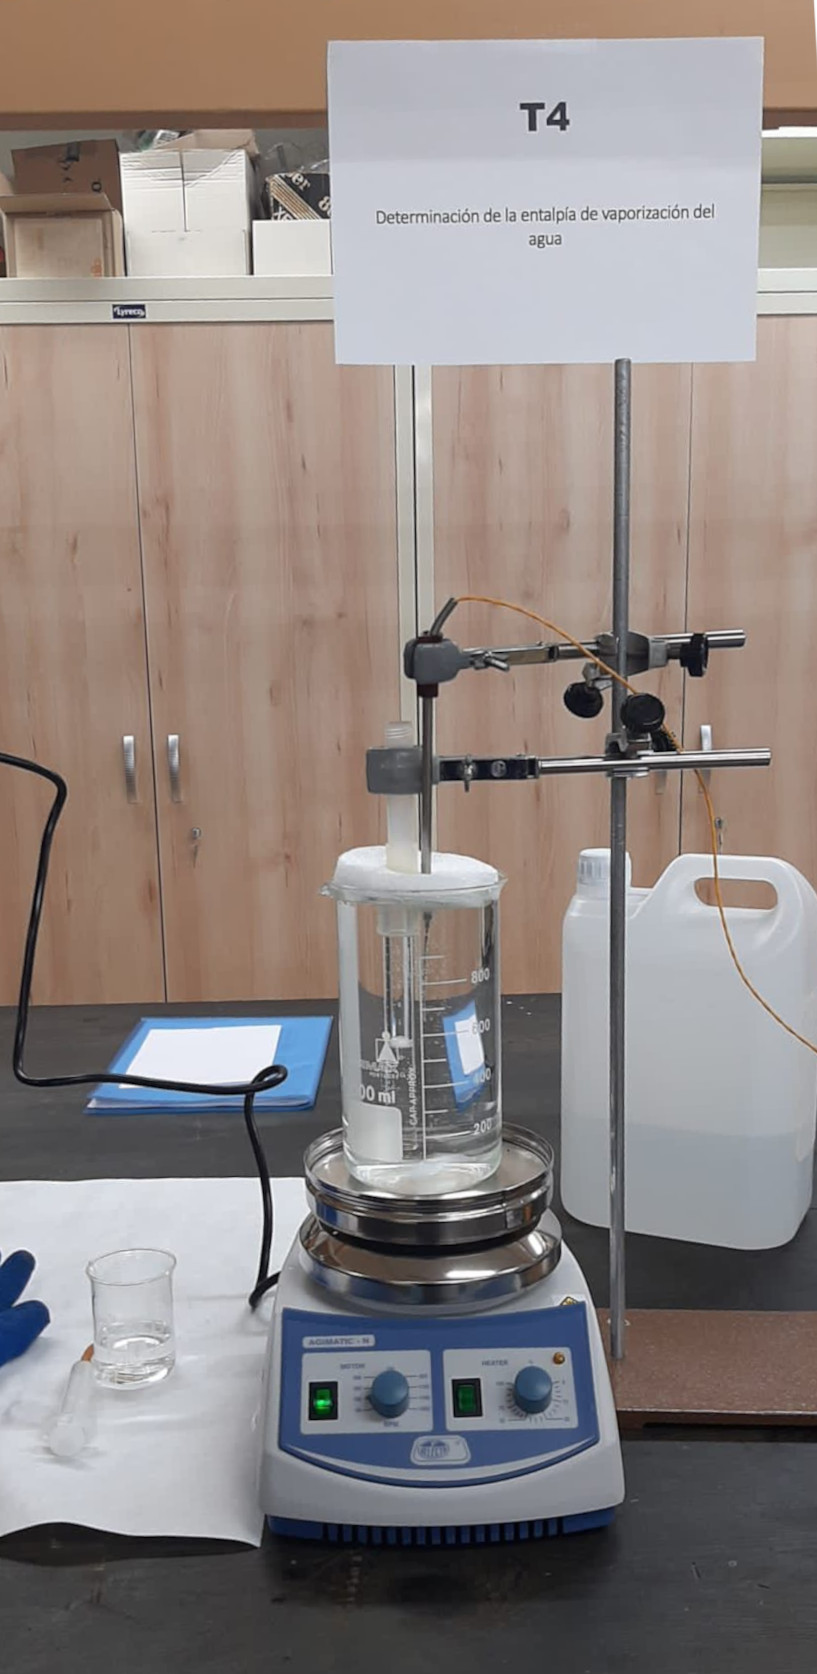
\includegraphics[width=.26\textwidth]{fotos/portada.jpeg}
    \end{wrapfigure}

    \hfill{}\\
    Els objectius d'aquest informe estan definits a el {\textit{abstract}}, estudiarem la relació de la pressió de vapor amb la temperatura per a verificar l'equació de Clausius-Clapeyron. Esta equació facilitarà el càlcul de tant l'entalpia de vaporització com de la temperatura d'ebullició de l'aigua. A més, finalment compararem les dades experimentals amb l'aproximació de Antoine.\\ \\La motivació principal és l'obtenció de dades experimentals més importants (des d'un punt de vista termodinàmic) del líquid més abundant al nostre planeta, l'aigua. I es que dades com el punt d'ebullició de l'aigua, que a primera vista puguen semblar obvies o d'escassa utilitat, han sigut molt importants per al desenvolupament industrial de la humanitat. Per eixemple, la certesa de la mesura en relació a la pressió es clau per a estalviar energia esterilitzant productes mitjançant l'ebullició d'aigua.\\ \\A fi de profunditzar en aquests resultats i aportar conclusions, realitzem aquest breu estudi sobre el tema.
    \vspace{0.5cm}

\section{Marc teòric}
    A aquest apartat discutirem les bases teòriques de l'inform en profunditat, començant amb l'energia lliure de Gibbs, denotada $G$.
    \begin{equation}\label{eq:gibbs}
    G\equiv H-TS    
    \end{equation}
    L'energia lliure de Gibbs, $G$, es un potencial termodinàmic que pot ser utilitzat per a calcular el màxim del treball reversible que pot realitzar-se mitjançant un sistema termodinàmic, a una temperatura y pressió constants.\\ \\Cal destacar que la variació d'aquest potencial soles dependrà dels estats inicial i final, no del camí entre els estats. A més, el treball realitzat es sempre menor a $G$ i soles serà igual si ens trobem a un procés reversible al qual no n'hi ha treball d'expansió. \\ \\Ara, continuarem definint el potencial químic, $\mu$.
    \begin{equation}\label{eq:potencial}
    \mu_i \equiv \left( \frac{\partial G}{\partial n_i} \right)_{T,P,n_{i\neq j}} = \left( \frac{\partial F}{\partial n_i} \right)_{T,V,n_{i\neq j}} = \left( \frac{\partial H}{\partial n_i} \right)_{S,P,n_{i\neq j}} = \left( \frac{\partial U}{\partial n_i} \right)_{S,V,n_{i\neq j}}
    \end{equation}
    El subíndex de l'equació ens indica que el potencial químic està associat a cada espècie. Per tant, el que $\mu$ representa es com va a cambiar l'energia del sistema si augmentem el nombre de partícules d'una especie específica del sistema, pero sense modificar la resta de variables d'estat. Podem relacionar $G$ i $\mu$ mitjançant la definició d'entalpia.
    \begin{equation}\label{eq:entalpia}
        G = H - TS = TS + \sum_{i=1}^{e}\mu_idn_i - TS = \sum_{i=1}^{e}\mu_idn_i
    \end{equation}
    \clearpage
    Ara, anem a definir la noció de fase, una regió de l'espai on les propietats fisico-químiques són constants. Anem a treballar amb la transició entre dos d'aquestes fases, a la qual n'hi ha una coexistència de dos estats d'agregació: líquid i sòlid. Es útil observar el diagrama de fases de l'aigua (veure figura \ref{fig:DiagramaFase}) per a comprendre millor el camp que estem treballant.
    \begin{figure}[h]
        \centering
        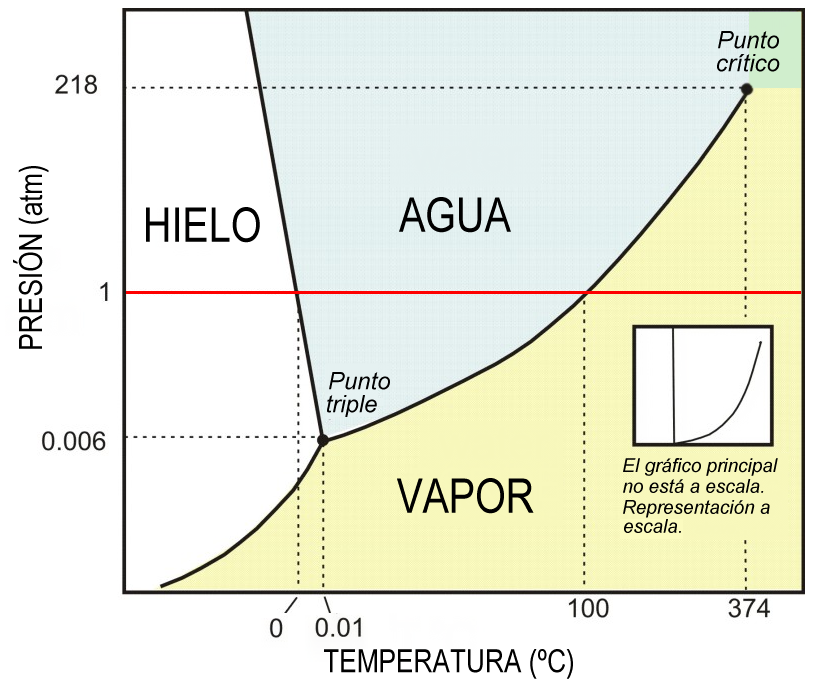
\includegraphics[width=.5\textwidth]{fotos/fase.png}
        \caption{Diagrama de fase de l'aigua}
        \label{fig:DiagramaFase}
    \end{figure}
    \hfill{}\\ 
    Anem a profunditzar en el canvi de fase. Podem observar que la pendent de la recta del canvi de fase sòlid-líquid es negativa, es a dir que l'aigua sòlida es menys densa que la líquida. Anem a tractar de mesurar la variació d'entalpia molar $\Delta\overline{H}$, a la transició de líquid-vapor. \\ \\Com el potencial químic es manté constant a la transició, podem dir que soles depenen de pressió i temperatura. $\mu_v\left(P,T\right)=\mu_l\left(P,T\right)$ Primerament, realitzem un canvi infinitesimal a la pressió i temperatura, que produirà un canvi infinitesimal a l'energia lliure de Gibbs. A més, com el nostre sistema soles pot produir treball degut a un canvi de volum arribem a que \[d\overline{G}=\overline{V}dP + \overline{S}dT\] comprovem que el canvi infinitesimal també manté que $d\mu_v\left(P,T\right)=d\mu_l\left(P,T\right)$ Com el potencial lliure de Gibbs molar coincideix amb el potencial químic quan estem al canvi de fase, deduïm que: \[\overline{V}_vdP + \overline{S}_vdT = \overline{V}_ldP + \overline{S}_idT \iff \frac{dP}{dT}=\frac{\overline{S}_v-\overline{S}_l}{\overline{V}_v-\overline{V}_l}=\frac{\Delta\overline{S}_vl}{\Delta\overline{V}_vl}\] Si apliquem la següent relació $\Delta\overline{S}=\frac{\Delta\overline{H}}{T}$ arribem a l'equació de Clausius-Clapeyron on $v$ denota vaporització. \[\frac{dP_v}{dT}=\frac{\Delta\overline{H}_v}{T\Delta\overline{V}_v}\]
\clearpage
\section{Procediment experimental}
    \subsection{Material}
    Ara, descriurem breument el material necessari per a realitzar l'experiment:
    \begin{multicols}{2}
        \begin{itemize}
            \item Vas de precipitats $1\si{\litre}$
            \item Tub d'assaig (amb divisions de $1\si{\milli\litre}$)
            \item Calefactor elèctric
            \item Agitador magnètic
            \item Termòmetre tipus termoparell
            \item Aigua destil·lada bullida
            \item Gel
            \item Xeringa
        \end{itemize}
    \end{multicols}
    
    \vspace{10pt}
    \subsection{Metodologia}
    L’experiment realitzat en el laboratori va consistir d'un recinte tancat (tub d’assaig donat la volta) on n'hi ha un gas (aire) en contacte amb un líquid (aigua destil·lada bullida) com podem observar a la figura.
    
    \begin{wrapfigure}{l}{.45\textwidth}
        \centering
        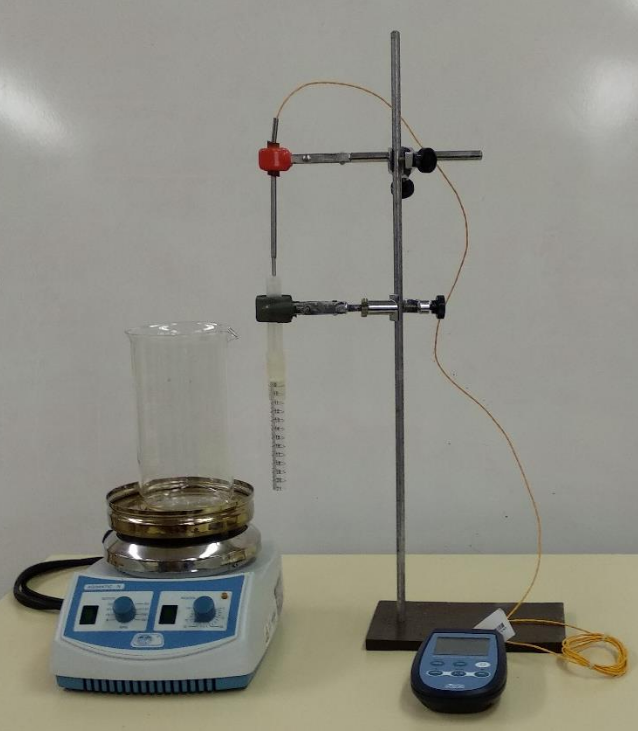
\includegraphics[width=.45\textwidth,height=9.5cm]{fotos/setup.png}
        \caption{Disposició experimental}
        \label{fig:Disposició experimental}
    \end{wrapfigure}

    \hfill{}\\
    A la figura \ref{fig:Disposició experimental} es mostra la disposició del material experimental que es va utilitzar. La fase gasosa, que es troba a l’interior del tub d’assaig, consisteix en una quantitat fixa d’aire i una variable de vapor d’aigua que variarà amb la temperatura de tot el sistema. Seguidament, es descriu com mesurar el volum de la fase gasosa en funció de la temperatura, que ens permetrà obtindre la pressió de vapor de l’aigua. Després d’aplicar l’equació de Clausius-Clapeyron obtindrem l’entalpia de vaporització. \\ \\En primer lloc s’ompli el vas de precipitat amb aigua destil·lada i es col·loca sobre el calefactor. A continuació, s'introdueix aigua destil·lada bullida en el tub d’assaig fins aproximadament $\frac{2}{3}$ del volum total, es tapa amb un dit l’extrem, i s’inverteix el tub d'assaig. Coloquem el tub en aquesta posició dins del vas de precipitat, amb cura de que quede completament submergit dins de l’aigua. S’ha d’utilitzar aigua destil·lada bullida prèviament per a omplir el tub d’assaig amb la finalitat d’evitar les bambolles d’aire que normalment són dissoltes a l'aigua. D’aquesta manera a l’interior del tub d’assaig es forma una càmera amb una mescla gasosa d’aire i vapor d’aigua. \\ \\ Aïllem el vas de precipitat de l’exterior, per a garantir l’equilibri tèrmic, i el tapem amb una planxa de poliuretà, a través de la qual es fa passar un termoparell que permet mesurar la temperatura de l’aigua i de la mescla gasosa de l’interior del tub d’assaig. El termoparell s’ha de situar de manera que l’extrem lliure es trobe pròxim al tub d’assaig i cap a la meitat d’aquest. S’encén el calefactor, al $40-50\%$ de la seua potència màxima, fins que l’aigua arribe a una temperatura aproximada de $65\si{\celsius}$. L’agitador ha d’estar activat a $200 \frac{\text{rev}}{\text{minut}}$ per a mantenir una distribució de temperatures homogènia a tot el sistema. 
    \newpage
    En aconseguir la temperatura de $65\si{\celsius}$, es deté el calefactor, encara que l’agitador ha de romandre actuant en tot moment. Llavors l’aigua es refredarà per convecció tèrmica. És important desconnectar el calefactor una vegada arribem a $65\si{\celsius}$ ja que el vidre del tub es trencarà a temperatures superiors. Seguidament es faran mesures del volum $V$ de la cambra gasosa de l’interior del tub d’assaig en funció de la temperatura $T$ per a totes les divisions possibles de l’escala del tub, en un rang entre $65\si{\celsius}$ i $50\si{\celsius}$.\\ \vspace{-0.65cm}

    \begin{wrapfigure}{r}{.45\textwidth}
        \centering
        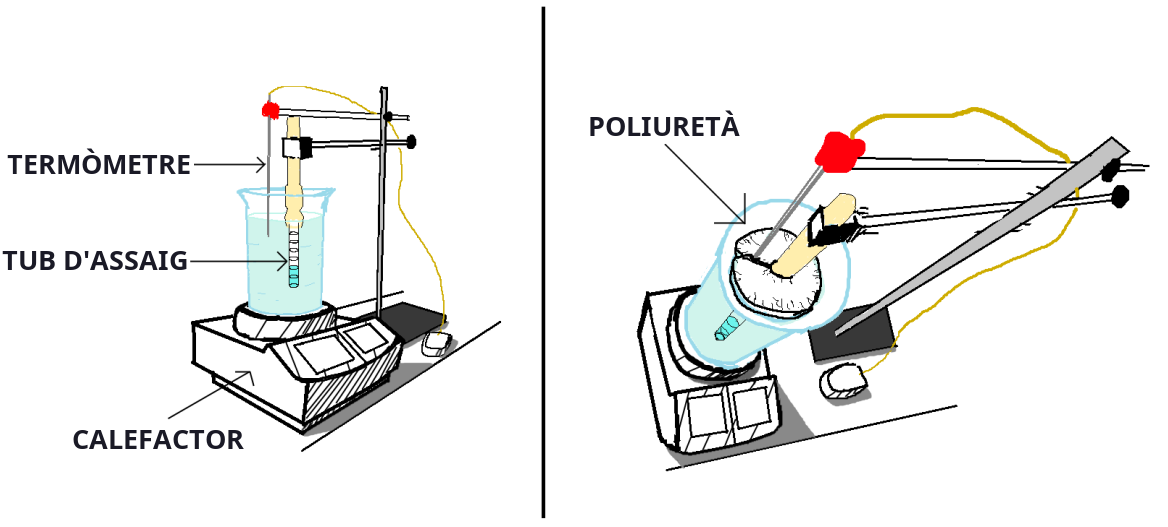
\includegraphics[width=.45\textwidth]{fotos/esquemaSetup.png}
        \caption{Esquema del material}
        \label{fig:esquema experimental}
    \end{wrapfigure}

    \hfill{}\\\hfill{}\\
    La mesura del volum del gas del tub d’assaig es fa per visualització directa del menisc de l’aigua a l’interior del tub d’assaig. La pressió total $P_{\text{mescla}}$ del sistema gasós de l’interior del tub d’assaig es considera aproximadament constant i igual a la pressió atmosfèrica, $P_0$, en l’interval de temperatures utilitzat en aquest experiment, menyspreant el pes de la columna d’aigua del tub. La pressió atmosfèrica al laboratori es mesura amb un baròmetre de mercuri. (veure apèndix \ref{appendix:baròmetre})

    
\section{Resultats i discussió}
    Procedim ara a expondre els resultats experimentals. Seguint els objectis parlarem de la medició de la pressió de vapor de l'aigua, de l'equació de Clausius-Clapeyron i de Antoine. 
    \subsection{Càlcul de la pressió de vapor de l'aigua}
        El primer pas lògic es calcular els valors de la pressió de vapor associats a les mesures experimentals. La pressió del laboratori $P_0$ va ser mesurada amb un baròmetre de Torricelli (veure apèndix \ref{appendix:baròmetre}) i vam obtindre un valor de $P_0 = (101820 \pm 7)\si{\pascal}$. Les taules amb les dades experimentals de la temperatura i el valumen es troben a l'apèndix \ref{appendix:dades}.\\ \\Calculem ara la pressió de vapor juntament amb el seu error corresponent mitjançant l'equació següent: \[P_v = P_0\left( 1-\frac{V_0T}{T_0V}\right)\]\label{eq:vapor} Els errors estan descrits a l'apèndix \ref{appendix:errors}. Ara, grafiquem les dades obtingudes.
        \begin{figure}[h]\label{fig:presio_de_vapor}
            \centering
            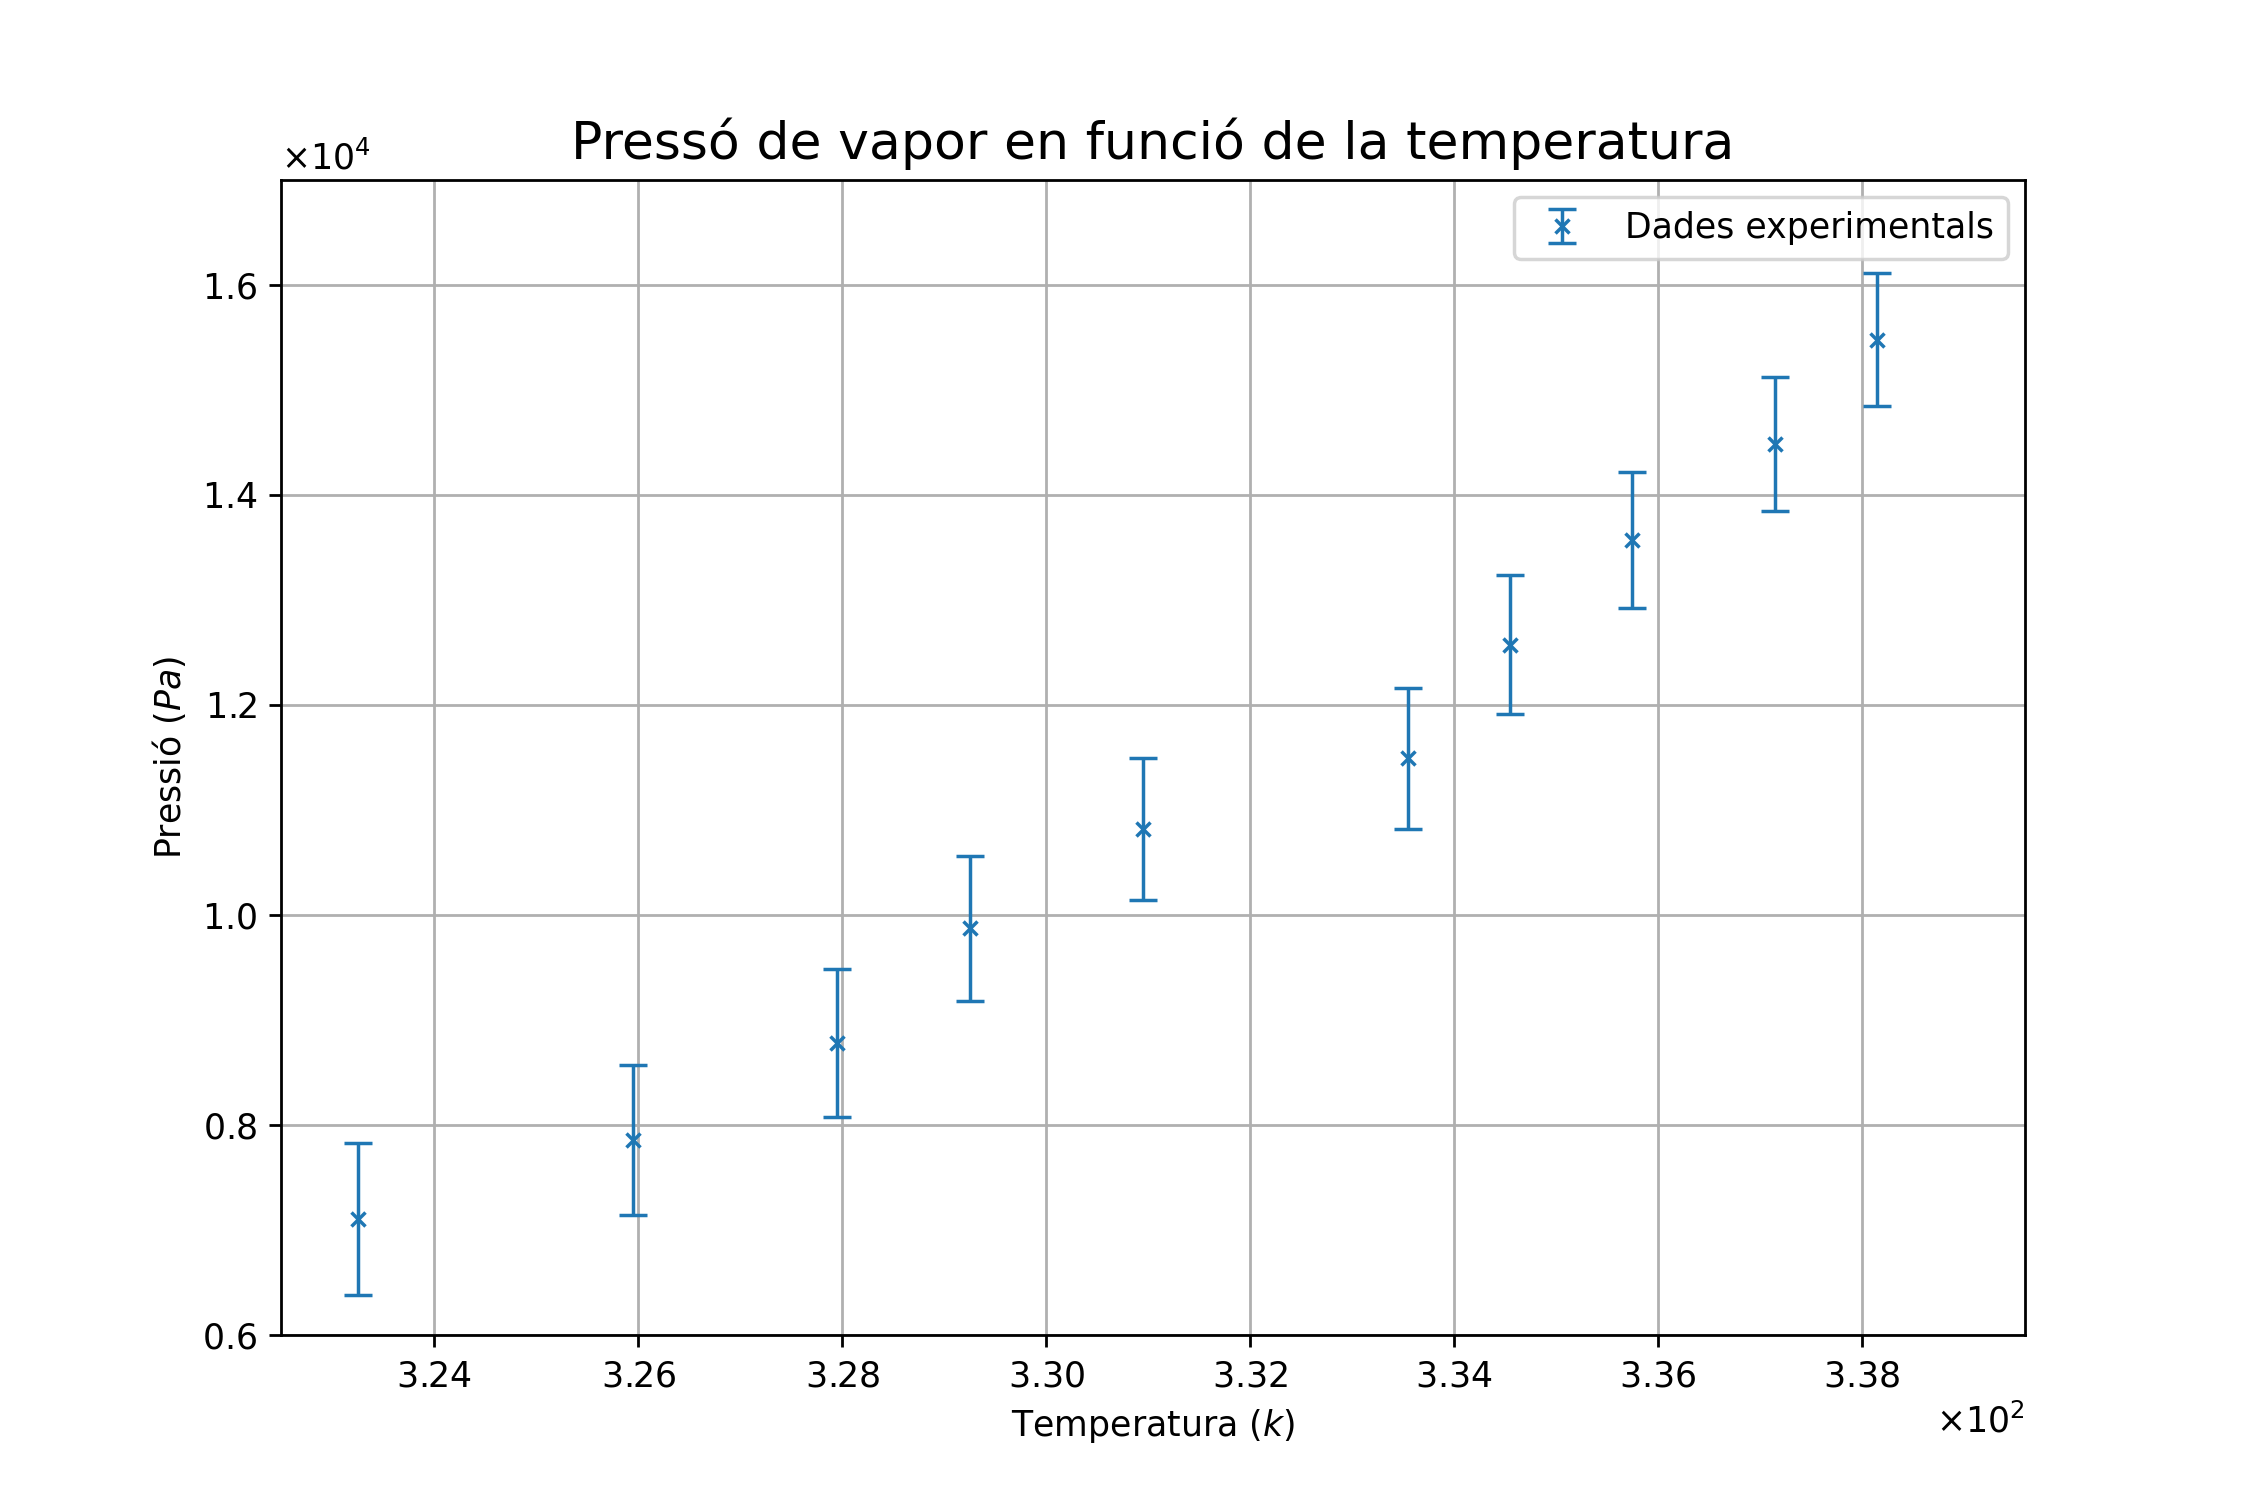
\includegraphics[width=.6\textwidth]{fotos/presionvapor.png}
            \caption{Pressió de vapor de l'aigua en funció de la temperatura}
        \end{figure}
        \clearpage
        Cap destacar que no podem veure l'error en la temperatura per ser molt petit en comparació amb l'error en la pressió.
        Per a la realització d'aquesta gràfica, hem suposat que la pressió de vapor de l'aigua a $0\si{\celsius}$ era de $0\si{\pascal}$. Però en la realitat sabem que el valor es de $610\si{\pascal}$. Hem de modificar \ref{eq:vapor} per a tindre en compte aquest apunt.\[P_v = P_0 - \frac{\left(P_0 - 610\right)V_0T}{T_0V}\]Graficant altra vegada, però amb les dades modificades,
        \begin{figure}[h]\label{fig:presio_de_vapor2}
            \centering
            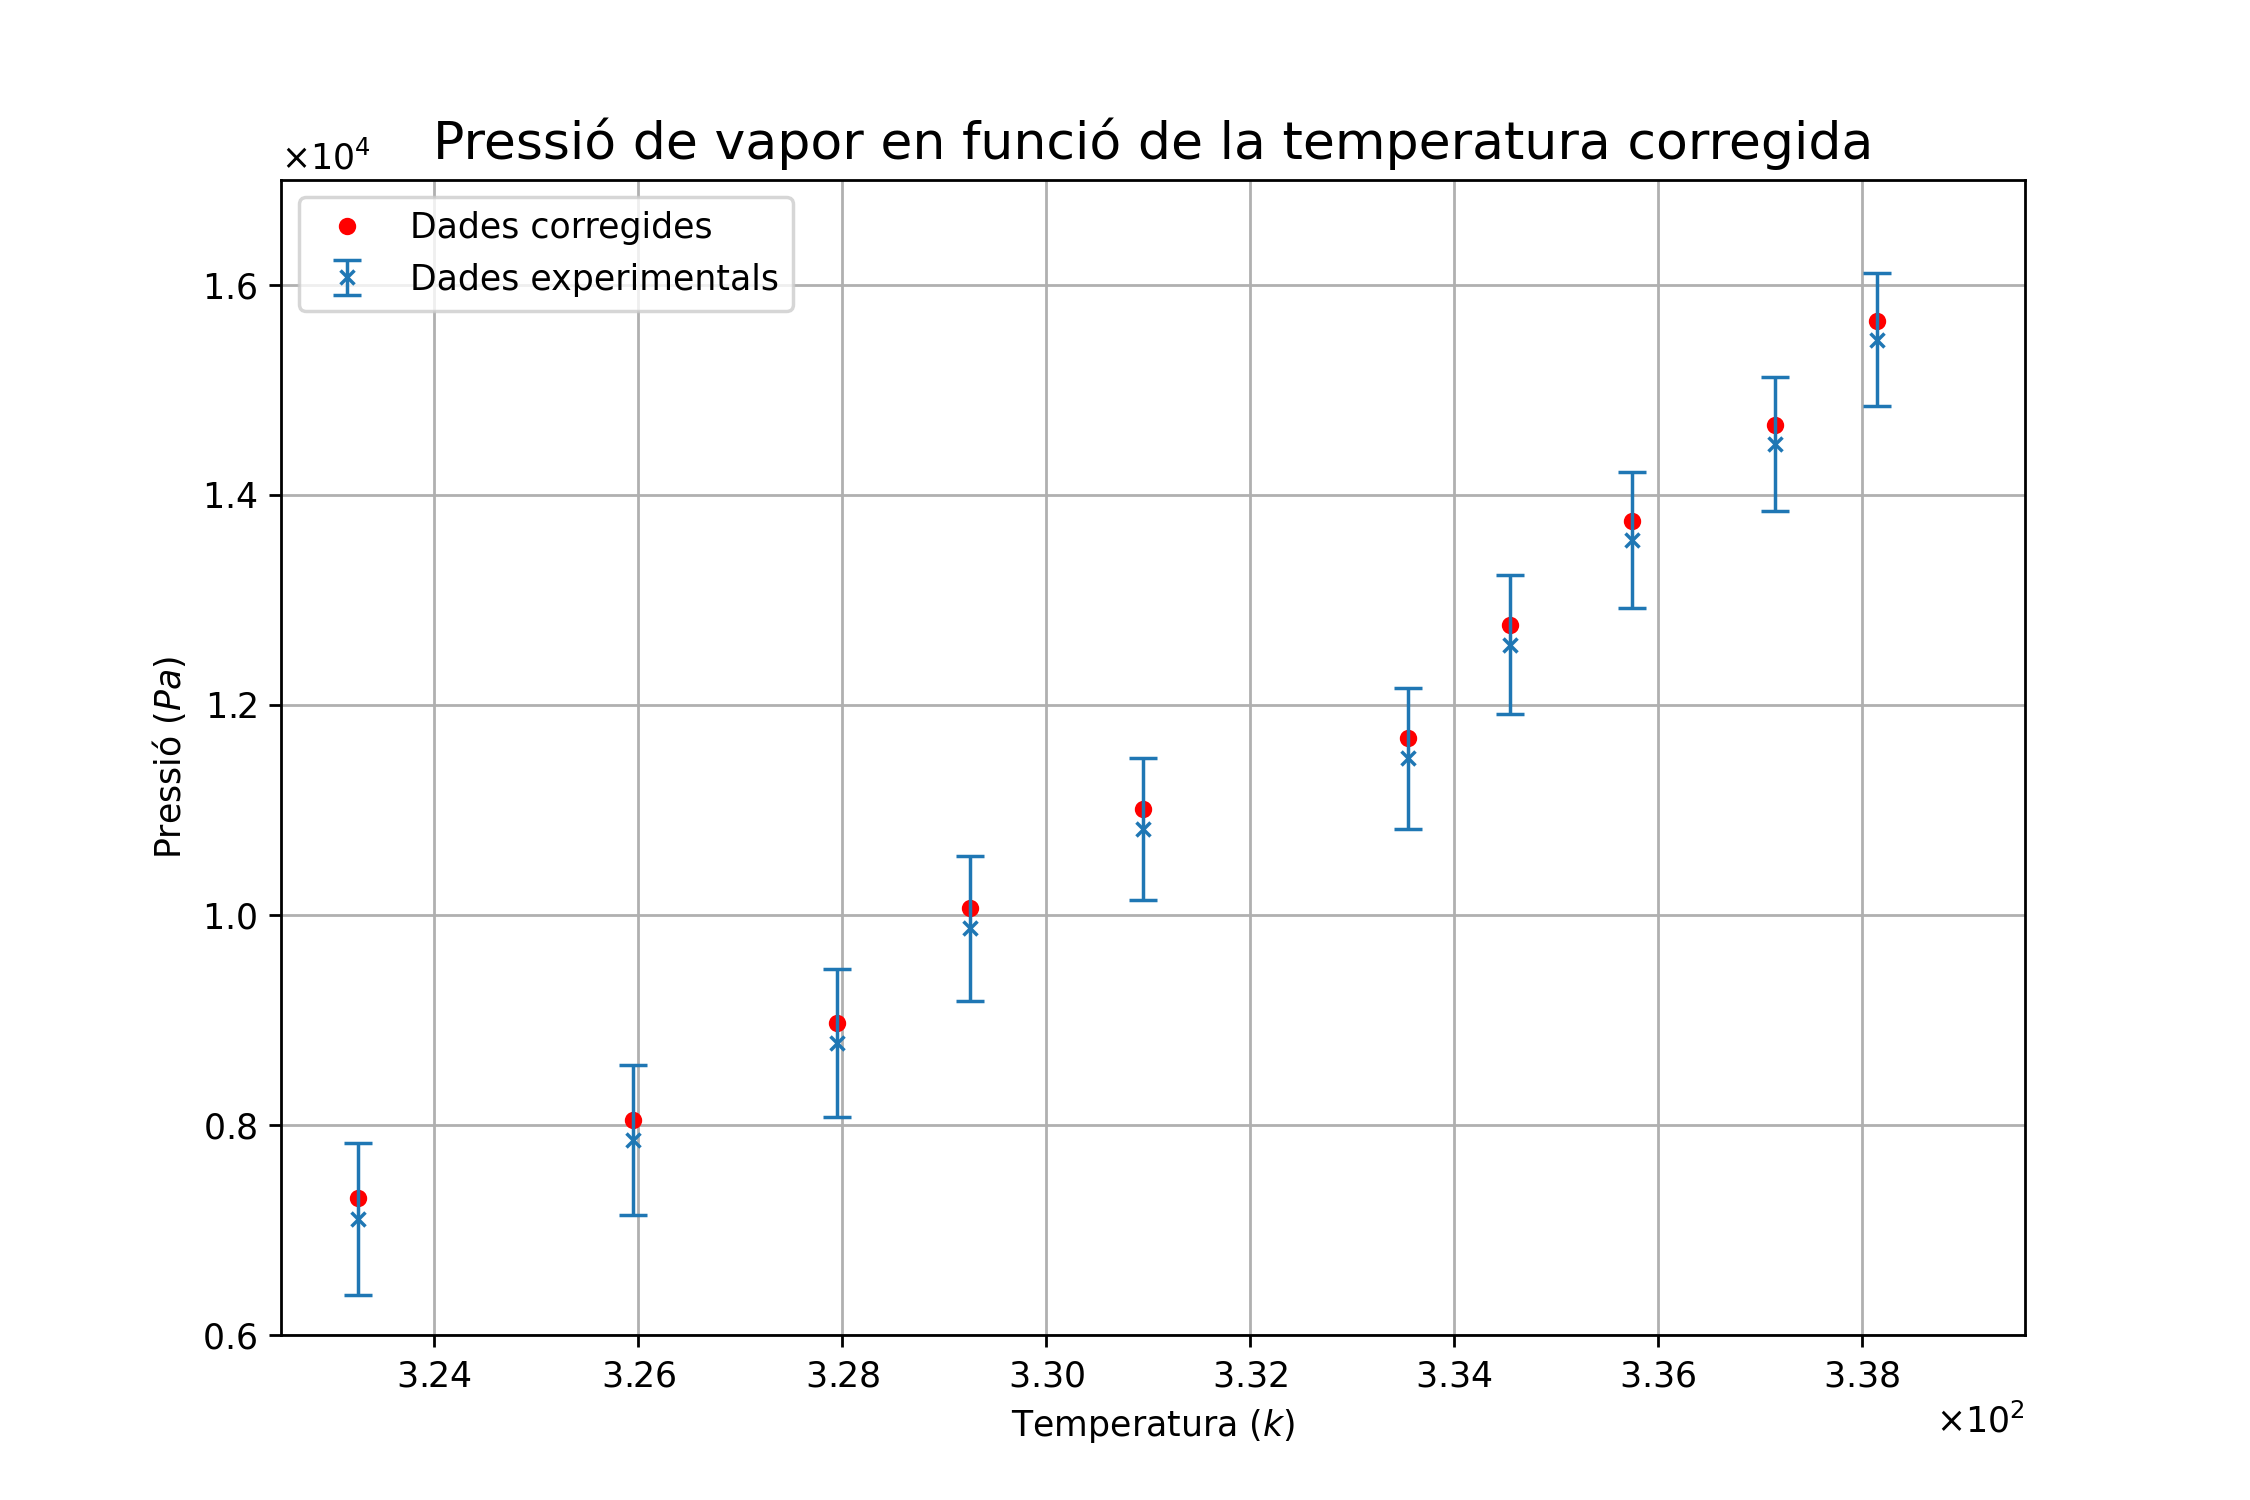
\includegraphics[width=.75\textwidth]{fotos/presionvapor2.png}
            \caption{Error al suposar que $P_v = 0$ en $T = 0\si{\celsius}$}
        \end{figure}
        \hfill{}\\
        Podem observar la diferència amb les nostres dades és quasi igual a tots els punts, i sempre dins de les barres d'error representades.

        \clearpage
    \subsection{Verificació de l'equació de Clausius-Clapeyron}
        Per a realitzar aquesta secció, necessitem primerament conèixer l'equació de Clausius-Clapeyron\[\log\left(\frac{P_v}{P_0}\right)=\frac{\Delta \overline{H}_v}{R}\left(\frac{1}{T_{0\ \text{eb}}}-\frac{1}{T}\right)\]\label{eq:Clausius}Com es trata d'una relació logarítmica, utilitzarem paper logarítmic per a la realització de la gràfica corresponent. Tindrem $\left(\frac{P_v}{P_0}\right)$ a l'eix $y$ amb el seu error corresponent, i en el eix $x$ $\frac{1}{T}$ també amb el seu error corresponent però no l'apreciarem ja que es massa petit. Linealitzant les dades i obtenint la pendent, tindrem un valor per a la relació $\log\left(\frac{P_v}{P_0}\right)$. Podem obtindre també l'increment d'entalpia molar de vaporització de l'aigua, així com la temperatura d'ebullició de l'aigua a la pressió atmosfèrica del laboratori.
        \begin{figure}[h]\label{fig:Clausius}
            \centering
            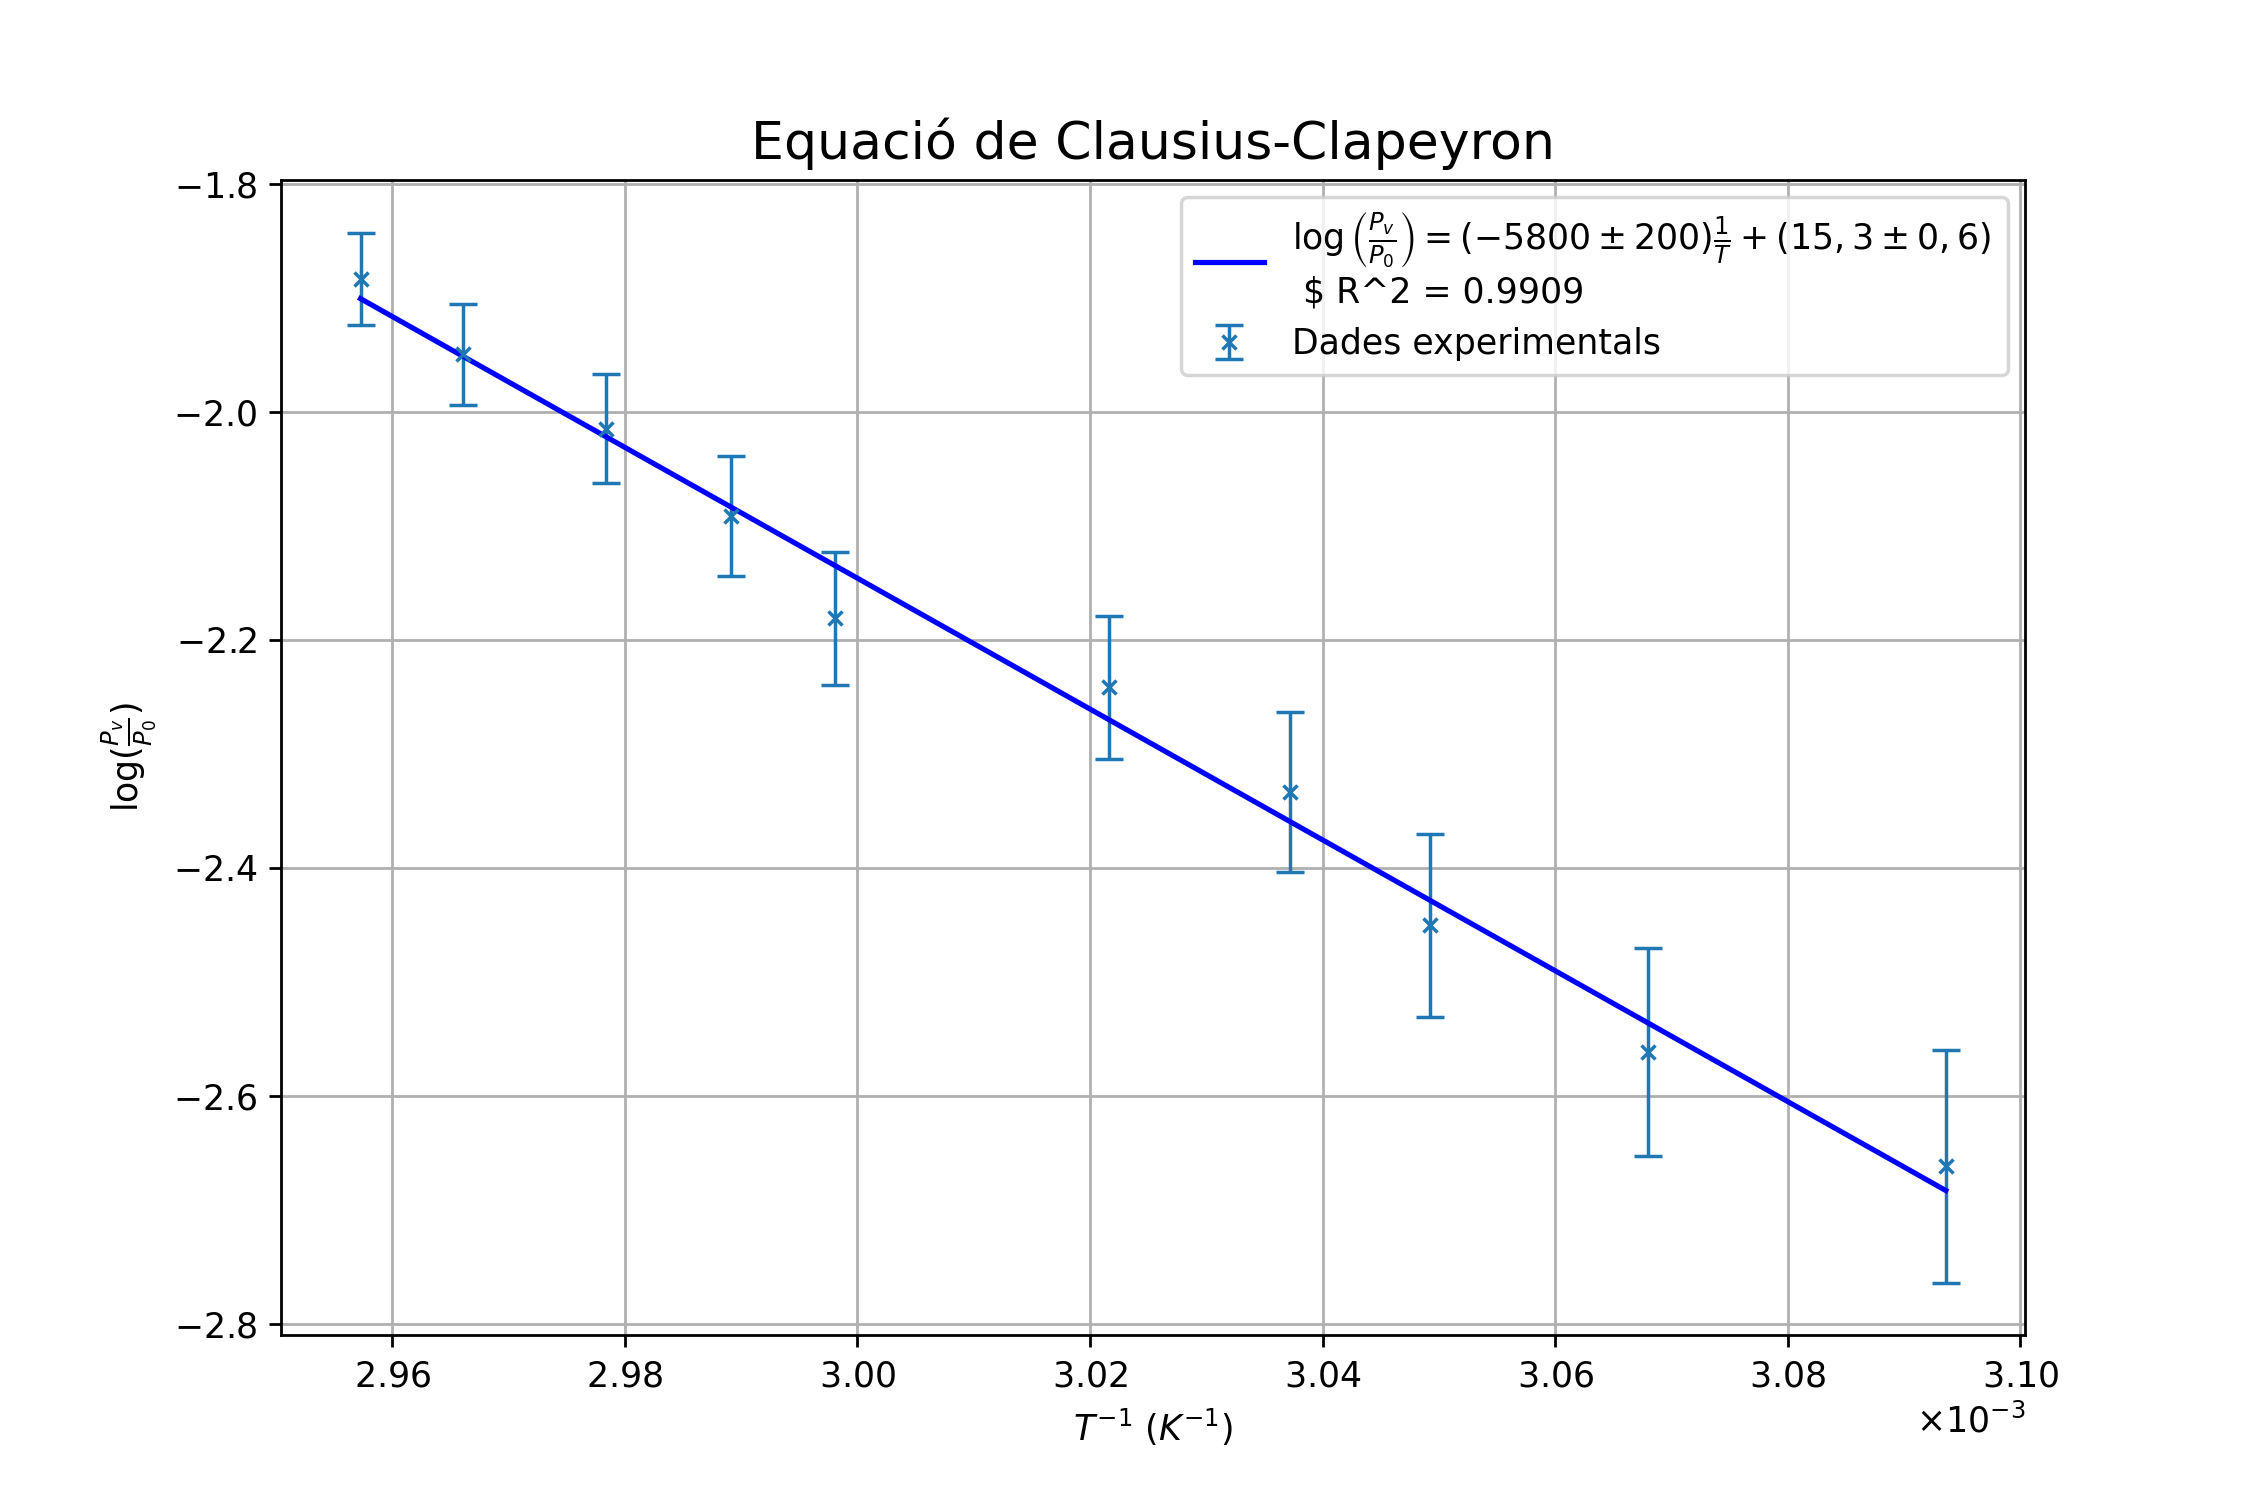
\includegraphics[width=.75\textwidth]{fotos/Clausius-Claperyon.png}
            \caption{Equació de Clausius-Clapeyron}
        \end{figure}
        \hfill{}\\
        Obtenim un $R^2$ molt proper a 1, que ens certifica que les dades poden aproximar-se amb una recta. Fixant-nos a l'equació \ref{eq:Clausius} podem realitzar els següents càlculs. \[\log\left(\frac{P_v}{P_0}\right)=\left(-5600\pm200\right)\frac{1}{T}+\left(15.3\pm0.6\right)=\frac{\Delta\overline{H}_v}{R}\left(\frac{1}{T_{0\ \text{eb}}}-\frac{1}{T}\right)\] D'aquest resultat podem obtindre el següent.\[-5800\pm200=\frac{\Delta\overline{H}_v}{R} \hspace{4cm} 15.3\pm0.6=\frac{\Delta\overline{H}_v}{RT_{0\ \text{eb}}}\] Per a finalment obtindre que: \[\Delta\overline{H}_v = -48200\pm1700\si{\joule}\text{/}\si{\mol} \hspace{4cm} T_{0\ \text{eb}} = 380 \pm 20 \si{\kelvin}\]Els errors d'aquests càlculs son a l'apèndix \ref{appendix:errors}, però cal destacar els errors relatius de ambdós, $3.5\%$ per a l'entalpia molar de vaporització de l'aigua, i $5.2\%$ per a la temperatura. Observem com l'error de la temperatura es més prominent que el de l'entalpia, encara que ambdós son relativament grans.
        
    
    \subsection{Comparació amb l'equació de Antoine}
    A aquesta secció anem a comparar les dades experimentals amb l'equació semi-empírica de Antoine. Aquesta equació té una forma diferent per a cada rang de temperatures, i específicament al nostre rang de temperatures (amb $P$ en \si{\kilo\pascal} i la resta en unitats del SI): \[\log\left(P_v\right)=16.573 - \frac{3988.842}{T - 39.47}\]
    Ara, graficarem aquesta aproximació amb les nostres dades experimentals per a obtindre la següent gràfica:
    \begin{figure}[h]\label{fig:antoine}
        \centering
        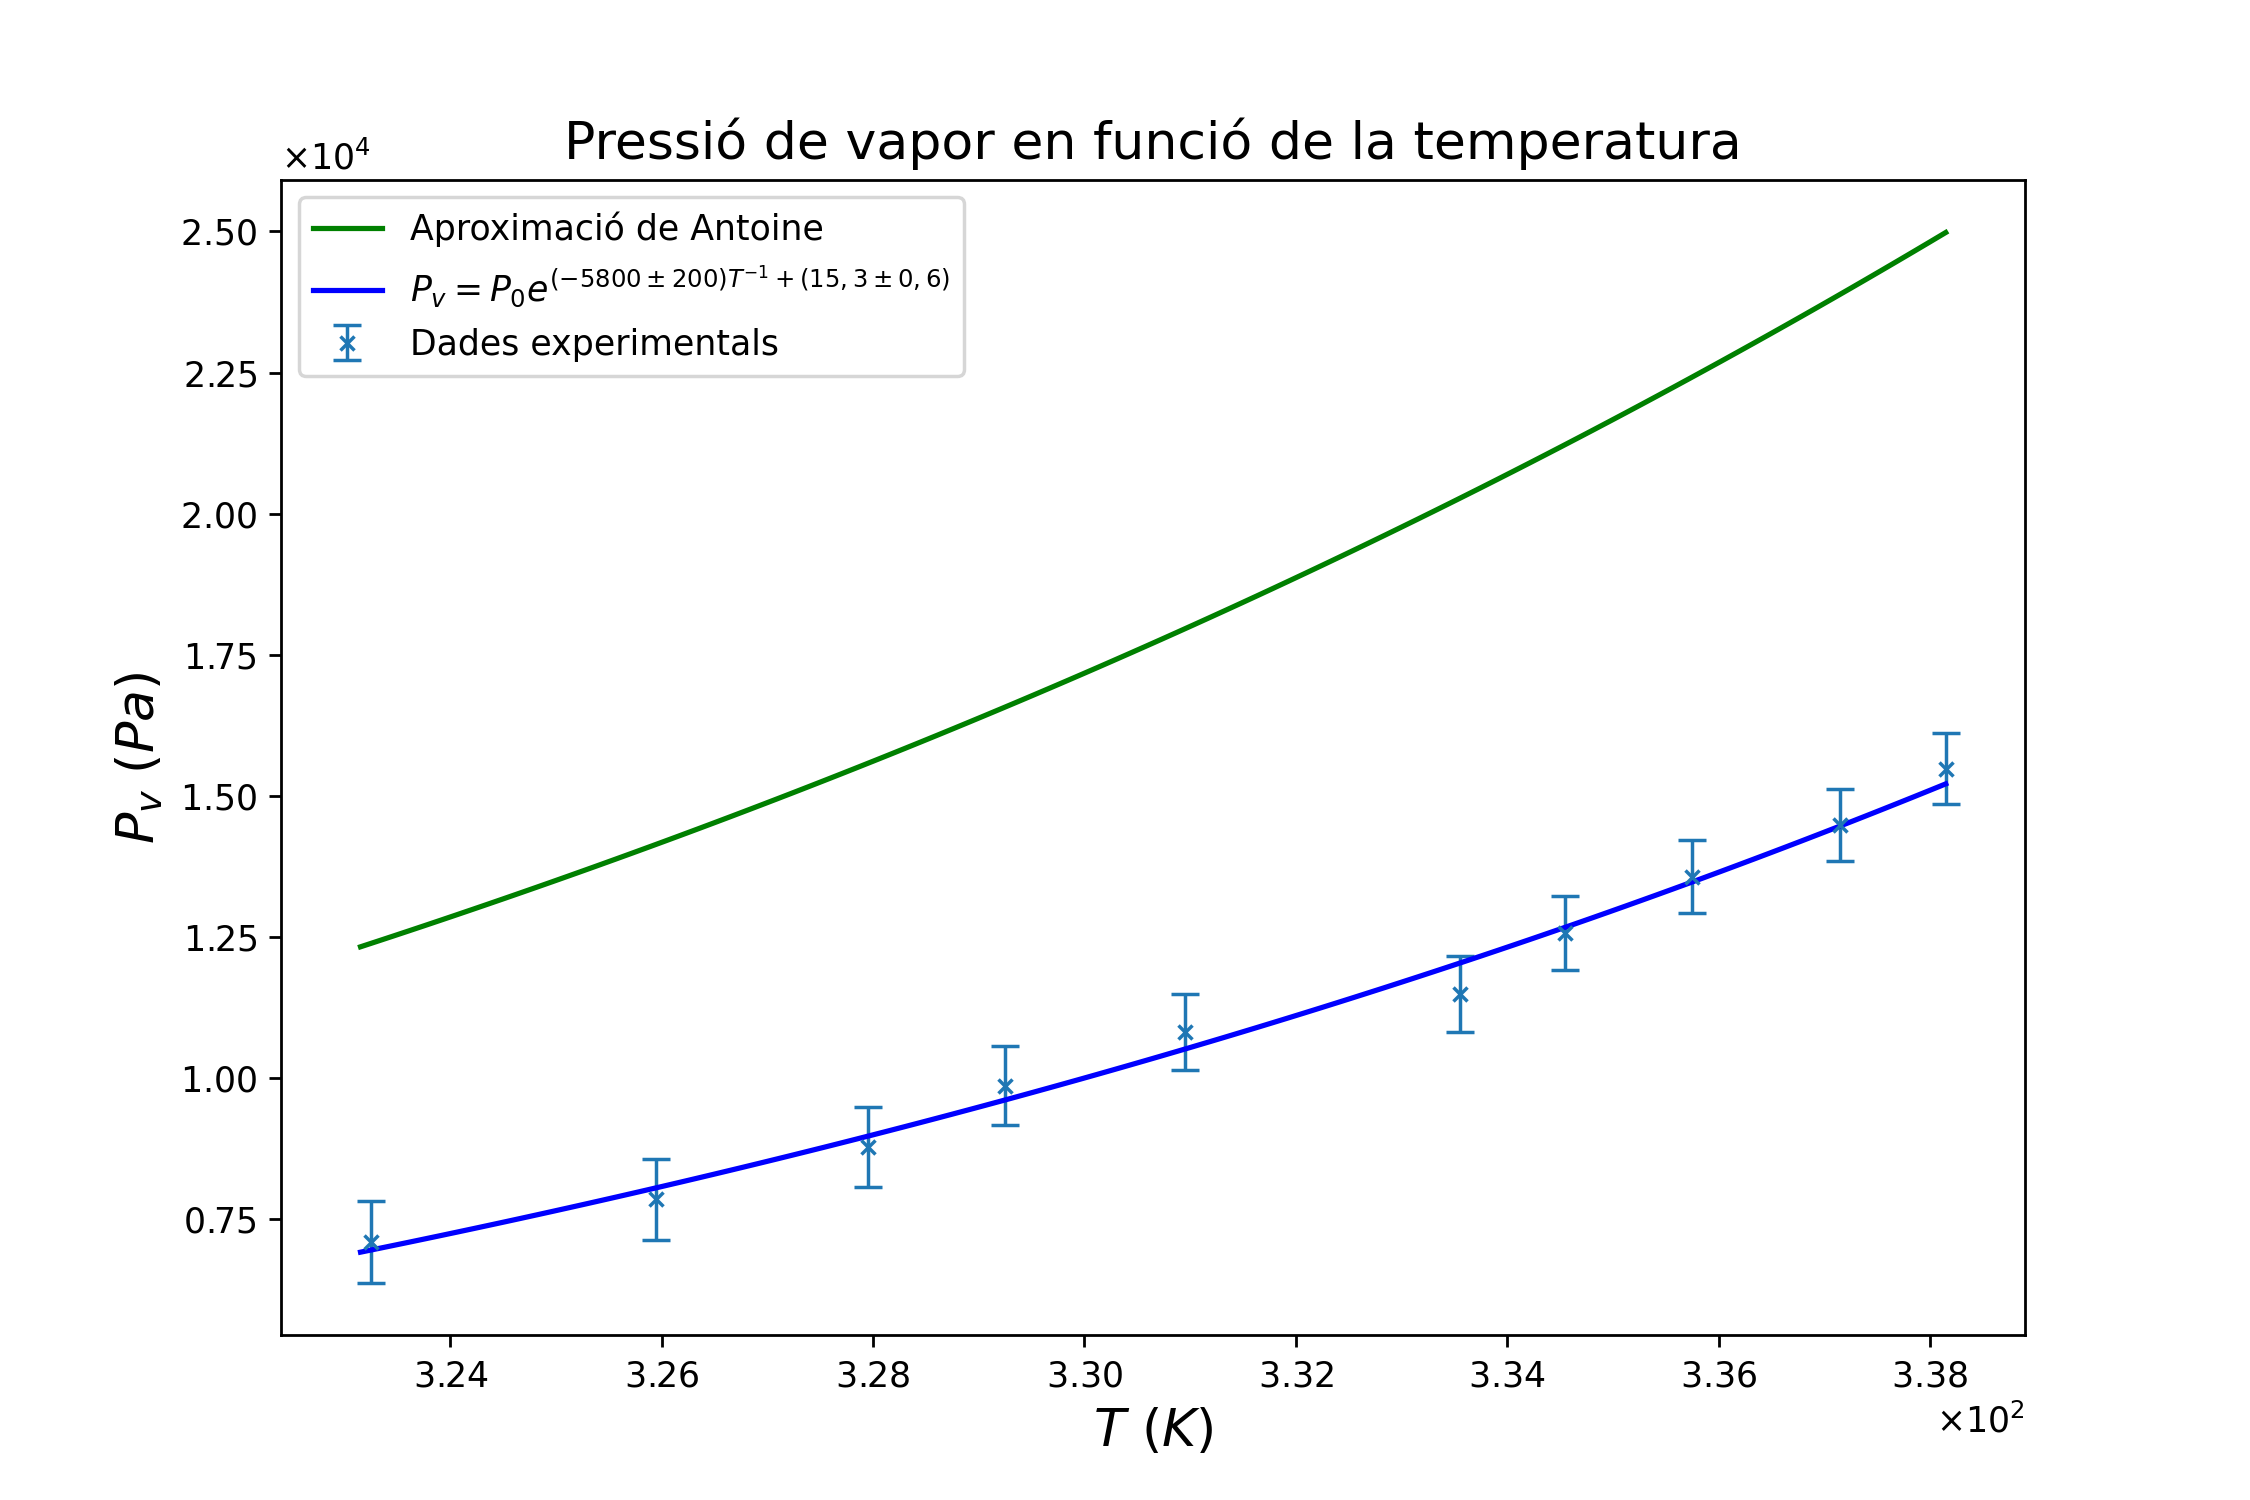
\includegraphics[width=0.55\textwidth]{fotos/antoine.png}
        \caption{Comparació experimental amb Antoine}
    \end{figure}
    Els nostres valors disten molt de l'equació de Antoine com podem observar. Això ens indica que n'hi ha un error a una suposició, tot i que la forma de l'aproximació es similar.\\ \\Ara, anem a calcular l'entalpia de vaporització i la temperatura d'ebullició desde l'equació semi-empírica de Antoine i arribem a la conclusió de que és una aproximació molt bona.\\ \\Aplicant el mateix desenvolupament matemàtic que a l'apartat de l'equació de Clausius-Clapeyron, obtenim els valors de: \[\Delta\overline{H}_v = -42767\pm8\si{\joule}\text{/}\si{\mol} \hspace{4cm} T_{0\ \text{eb}} = 372 \pm 0.014 \si{\kelvin}\] Comprovem que els errors son molt menuts en comparació amb els obtinguts experimentalment. La temperatura d'ebullició entra dins de l'error que hem marcat, però l'entalpia de vaporització s'allunya massa de les nostres barres d'error. Això torna a indicar-nos que n'hi ha una suposició que no es correcta.
    \begin{figure}[h]
        \centering        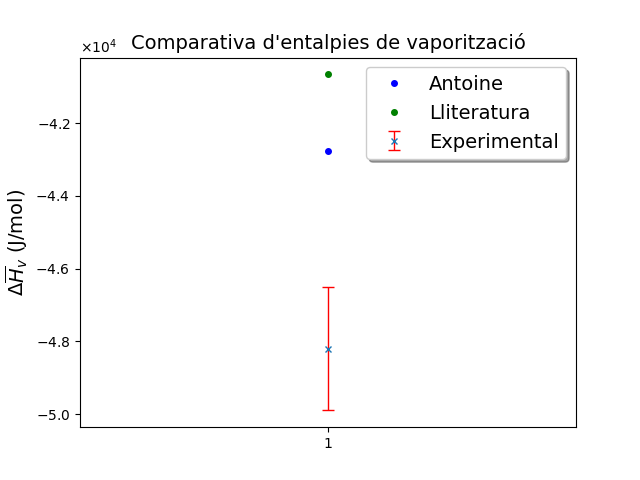
\includegraphics[width=0.4\textwidth]{fotos/entalpies.png}        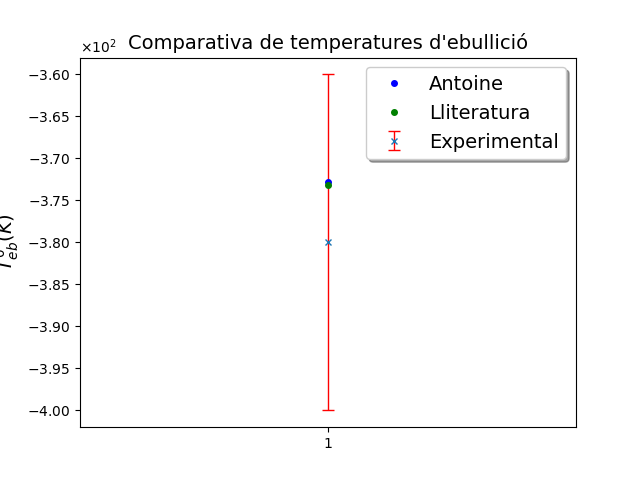
\includegraphics[width=0.4\textwidth]{fotos/temperatures.png}
    \end{figure}
\section{Possibilitats de millora}
    En aquesta secció profunditzarem en les causes dels errors experimentals, i com suprimir-los o minimitzar-los el màxim possible. Els errors més rellevants son l'error instrumental, l'error per la suposició de que la pressió de vapor es nula a $0\si{\celsius}$ i l'error per la suposició de que el vapor d'aigua es un gas ideal. L'error humà també es present però no hauria de ser molt significatiu sempre i quan no n'hi haja un error greu.\\ \\Si calculem els errors relatius, com està detallat a l'apèndix \ref{appendix:errors} observem que l'error en el volum es el major de tots que, juntament amb la suposició de que la pressió de vapor es nula a $0\si{\celsius}$ son els mes significatius. Probablement una forma més sofisticada i precisa de mesurar el volum ajudaria a que els valors experimentals s'apoparen més a l'equació semi-empírica de Antoine.
\section{Conclusions}
    Al nostre informe hem calculat primerament la pressió de vapor d'aigua, i amb aquesta dada, hem calculat la temperatura d'ebullició de l'aigua a pressió atmosfèrica, juntament amb l'entalpia de vaporització molar de l'aigua. La suposició de que l'aigua en estat gasós es un gas ideal i de que la pressió de vapor de l'aigua a $0\si{\celsius}$ és 0, han introduït unes imprecisions considerables.

\newpage
\section{Apèndixs}
    \subsection{Mesures amb baròmetre de mercuri}\label{appendix:baròmetre}
        \begin{wrapfigure}{l}{.45\textwidth}
            \centering
            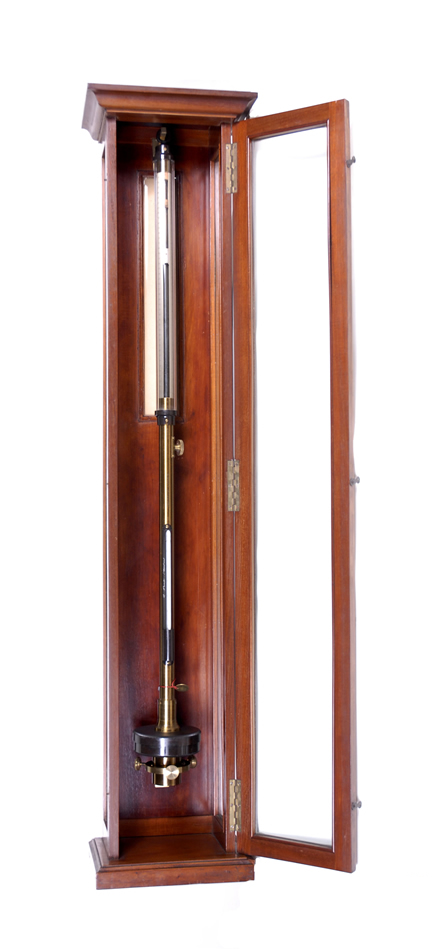
\includegraphics[width=.45\textwidth,height=9cm]{fotos/torricelli.png}
            \caption{Baròmetre de Torricelli}
            \label{fig:baròmetre}
        \end{wrapfigure}
        
        \hfill{}\\\hfill{}\\\hfill{}\\
        Evangelista Torricelli (1608-1647) va ser un físic italià que va inventar el baròmetre de mercuri, a més de demostrar que era possible tindre un recipient sense contingut al extraure l'aire del recipient. A la figura \ref{fig:baròmetre} podem veure aquest tipus de baròmetre, que es el utilitzat al laboratori.\\ \\
        Per a fer les mesures, en primer lloc s’ha de comprovar que la punta de la part inferior del baròmetre toca lleugerament el mercuri. A continuació, s’ha d’enrasar el menisc superior del mercuri amb el caragol superior , la pressió (en $\si{\deci\meter}$ de \ce{Hg}) es llegirà en l’escala de la dreta corresponent al valor del zero de la part superior del caragol metàl·lic. A aquesta pressió, hem de de restar-li la correcció corresponent a la temperatura que el fabricant ens facilita amb la taula de la figura \ref{fig:tabla}.\\ 

        \vspace{1cm}
        \begin{figure}[h]
            \centering
            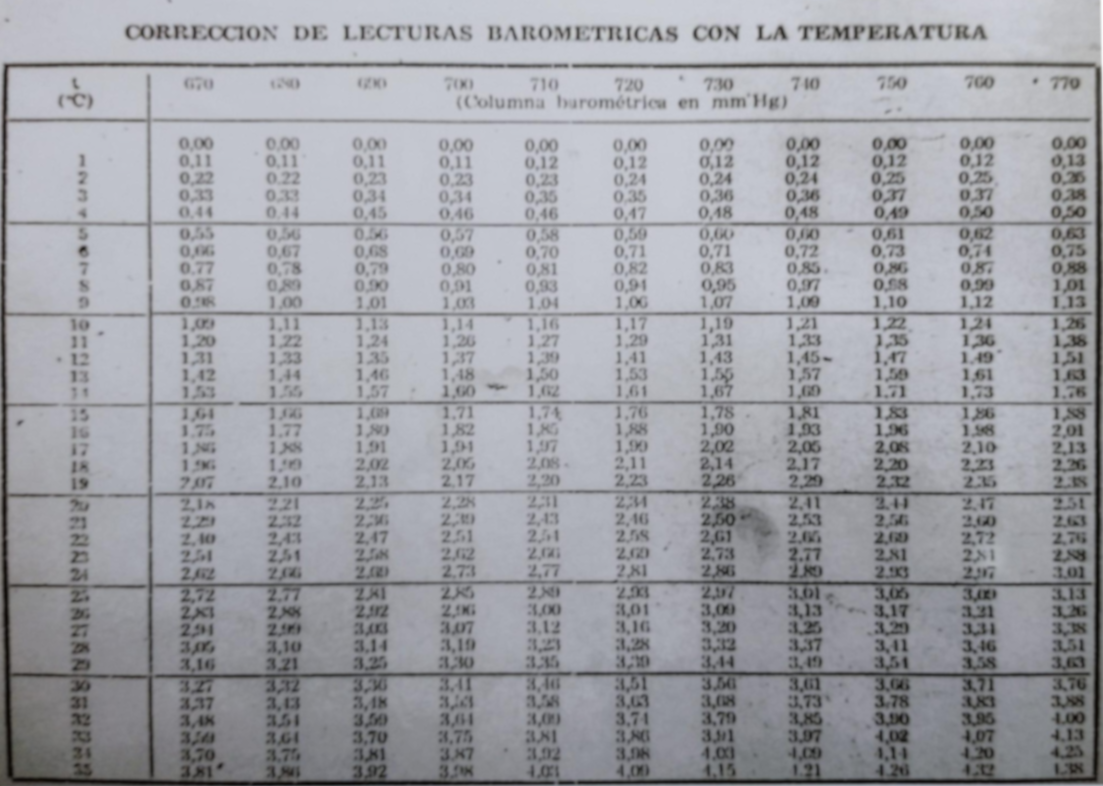
\includegraphics[width=.79\textwidth]{fotos/tablaBarometro.png}
            \caption{Tabla de correcció del baròmetre de Torricelli}
            \label{fig:tabla}
        \end{figure}
        \clearpage
    \subsection{Dades experimentals}\label{appendix:dades}
        A la taula \ref{tab:dades} podem vore les mesures experimentals tant de la temperatura com del volum del sistema termodinàmic.
        \begin{table}[h]\centering\label{tab:dades}\caption{Dades experimentals}
            \begin{tabular}{|cc|}
                \hline
                \rowcolor[HTML]{9698ED} 
                \textbf{$\left( T \pm 0.05\right) \si{\kelvin}$} & \textbf{$\left( V \pm 0.05\right) \cdot 10^{-6} \si{\meter}^3$} \\ \hline
                \rowcolor[HTML]{FFFFFF} 
                65                                               & 7                                                               \\
                \rowcolor[HTML]{DAE8FC} 
                64                                               & 6.9                                                             \\
                \rowcolor[HTML]{FFFFFF} 
                62.6                                             & 6.8                                                             \\
                \rowcolor[HTML]{DAE8FC} 
                61.4                                             & 6.7                                                             \\
                \rowcolor[HTML]{FFFFFF} 
                60.4                                             & 6.6                                                             \\
                \rowcolor[HTML]{DAE8FC} 
                57.8                                             & 6.5                                                             \\
                \rowcolor[HTML]{FFFFFF} 
                56.1                                             & 6.4                                                             \\
                \rowcolor[HTML]{DAE8FC} 
                54.8                                             & 6.3                                                             \\
                \rowcolor[HTML]{FFFFFF} 
                52.8                                             & 6.2                                                             \\
                \rowcolor[HTML]{DAE8FC} 
                50.1                                             & 6.1                                                             \\ \hline
            \end{tabular}
        \end{table} 
    \subsection{Càlcul d'errors}\label{appendix:errors}
        A aquest apèndix anem a calcular els errors, començant primerament amb els errors instrumentals, que seran: \[\mu\left(T\right)=\mu\left(T_0\right)=\frac{0.05}{\sqrt{3}}K \hspace{30mm} \mu\left(V\right)=\mu\left(V_0\right)=\frac{0.05}{\sqrt{3}}\cdot 10^{-6}\si{\meter}^3\hspace{30mm}\mu\left(P\right)=\frac{7}{\sqrt{3}}\si{\pascal}\] i amb propagació d'errors arribar a:\[\mu\left(P_v\right)=\sqrt{\left(\left(1-\frac{V_0T}{T_0V}\right)\mu\left(P_0\right)\right)^2+\left(\frac{P_0V_0T}{T_0V^2}\mu\left(V\right)\right)^2+\left(\frac{P_0V_0}{T_0V}\mu\left(T\right)\right)^2\left(\frac{P_0T}{T_0V}\mu\left(V_0\right)\right)^2\left(\frac{P_0V_0T}{T_0^2V}\mu\left(T_0\right)\right)^2}\]Aplicant la fòrmula al les dades experimentals, obtenim la següent taula:
        \begin{table}[h]\caption{Dades experimentals amb errors}
            \centering
            \begin{tabular}{|cc|}
            \hline
            \rowcolor[HTML]{9698ED} 
            \textbf{$\left(T\pm0.05\right)\si{\kelvin}$} & \textbf{$P_v\si{\pascal}$}       \\ \hline
            \rowcolor[HTML]{FFFFFF} 
            65.00                                        & $\left(154\pm6\right)\cdot 10^2$ \\
            \rowcolor[HTML]{DAE8FC} 
            64.00                                        & $\left(144\pm6\right)\cdot 10^2$ \\
            \rowcolor[HTML]{FFFFFF} 
            62.60                                        & $\left(135\pm6\right)\cdot 10^2$ \\
            \rowcolor[HTML]{DAE8FC} 
            61.40                                        & $\left(125\pm7\right)\cdot 10^2$ \\
            \rowcolor[HTML]{FFFFFF} 
            60.40                                        & $\left(114\pm7\right)\cdot 10^2$ \\
            \rowcolor[HTML]{DAE8FC} 
            57.80                                        & $\left(107\pm7\right)\cdot 10^2$ \\
            56.10                                        & $\left(98\pm7\right)\cdot 10^2$  \\
            \rowcolor[HTML]{DAE8FC} 
            54.80                                        & $\left(87\pm7\right)\cdot 10^2$  \\
            52.80                                        & $\left(78\pm7\right)\cdot 10^2$  \\
            \rowcolor[HTML]{DAE8FC} 
            50.10                                        & $\left(70\pm7\right)\cdot 10^2$  \\ \hline
            \end{tabular}
        \end{table}
        \clearpage
    \subsection{Comparació d'entalpies de vaporització}\label{appendix:entalpies}
        A aquest apèndix anem a comparar les entalpies de vaporització de diverses substancies, i observem que l'aigua es la substància amb menor entalpia de vaporització i anàlogament l'heli té una entalpia molt alta. Aquests valors ens indiquen la quantitat d'energia que hem d'aplicar a les substàncies per a que canvien de fase.

        \begin{table}[h]\centering\caption{Entalpies de vaporització}
            \begin{tabular}{cc|}
            \cline{2-2}
            \multicolumn{1}{c|}{\textbf{}}                        & \cellcolor[HTML]{9698ED}\textbf{$\Delta\overline{H}_v\si{\joule}\text{/}\si{\mol}$} \\ \hline
            \rowcolor[HTML]{FFFFFF} 
            \multicolumn{1}{|c}{\cellcolor[HTML]{FFFFFF}Aigua}    & -40656                                                                              \\
            \rowcolor[HTML]{DAE8FC} 
            \multicolumn{1}{|c}{\cellcolor[HTML]{DAE8FC}Metanol}  & -35300                                                                              \\
            \rowcolor[HTML]{FFFFFF} 
            \multicolumn{1}{|c}{\cellcolor[HTML]{FFFFFF}Acetona}  & -32000                                                                              \\
            \rowcolor[HTML]{DAE8FC} 
            \multicolumn{1}{|c}{\cellcolor[HTML]{DAE8FC}Butano}   & -21000                                                                              \\
            \rowcolor[HTML]{FFFFFF} 
            \multicolumn{1}{|c}{\cellcolor[HTML]{FFFFFF}Hidrogen} & -460                                                                                \\
            \rowcolor[HTML]{DAE8FC} 
            \multicolumn{1}{|c}{\cellcolor[HTML]{DAE8FC}Heli}     & -84.5                                                                               \\ \hline
            \end{tabular}
        \end{table}
    \subsection{Càlcul de les gràfiques}
        A aquest apèndix trobem el codi que he utilitzat per a fer les gràfiques
        \lstinputlisting[language=Python, firstline = 1]{graficas4.py}
\section{Referències}
    \hyperlink{https://webbook.nist.gov/chemistry/}{NIST Chemistry Book}\\ \\
    Apuntes de termodinámica, J.M. Villaplana Soria\\ \\
     \hyperlink{https://www.liceoagb.es/quimigen/liqu7.html}{liceoagb.es - Líquidos y sólidos, diagramas de fase}    
\end{document} 